% chapters/chapter2.tex  — converted from chapter2.typ
% Conventions used (identical to chapter1.tex):
%   Typst @KEY            -> \ac{KEY}        (auto: long on first use, short after)
%   Typst @KEY:pls        -> \acsp{KEY}      (short plural, e.g. "AVs")
%   Typst @figlabel       -> Figure~\ref{fig:figlabel}
%   Typst @citekey        -> \cite{citekey}
%   Typst @ch3[Chapter]   -> Chapter~\ref{ch3}
%   Typst @app:b          -> Appendix~\ref{app:b}
% Inside captions \acs{} is used so float placement cannot disturb first-use timing.
%
% NOTE: \ref{ch3} and \ref{app:b} need matching \label{ch3} (chapter3.tex) and
%       \label{app:b} (the appendix in main.tex) to resolve. Add them if missing.

\chapter{Interface Co-Simulation Design}
\label{ch2}

\section{Selecting the Suitable Simulator}
The development and testing of autonomous driving technologies require a robust simulation environment. This environment must accurately model the real world, including vehicles, pedestrians, and various environmental conditions, while also providing comprehensive support for sensor simulation and enabling integration with analytical tools. After a detailed evaluation of existing simulators, including the Waymo Simulator, LGSVL Simulator, Sim4CV, and CARLA Simulator, based on critical features such as graphic quality, the accuracy of the physics engine, sensor simulation capabilities, the simulation of traffic and pedestrians, weather conditions, the ability to simulate different times of day, CARLA Simulator has been identified as the most suitable choice for my research objectives. CARLA provides high-quality graphics with Unreal Engine 4~\cite{unreal_engine_4} and its physics engine accurately models vehicle dynamics and environmental interactions, offering a solid foundation for testing autonomous driving algorithms under various conditions. Moreover, its ability to simulate a wide range of sensors used in \acsp{AV}, such as cameras, LIDAR, radar, and GNSS, with high fidelity is crucial for the development and testing of perception algorithms. CARLA also excels in simulating dynamic traffic scenarios and pedestrian behaviors, facilitating comprehensive testing of autonomous driving systems in complex urban environments. The capability to simulate different weather conditions and times of day is important for assessing the performance of \ac{AV} systems under various environmental conditions. For my research, Python API of CARLA facilitates easy integration with an external controller, providing a seamless workflow for data analysis and algorithm testing. Consequently, CARLA Simulator's advanced graphics, accurate physics engine, extensive sensor simulation capabilities, and effective traffic and pedestrian simulation set it as the ideal choice for my autonomous driving research. Its compatibility with Python API further supports my analytical and development needs, making it the most suitable simulator for my project.

\section{Modeling the Car in the Environment}
In order to control a vehicle in the simulation, the controller must recognize the vehicle model. For this, a model of the vehicle is needed. Various models can be used when modeling the vehicle. Among these, the most commonly used ones usually offer a good balance between simplicity and accuracy, capable of representing the vehicle's motion dynamics and control systems. In line with the needs of this project, the \ac{DST} model has been chosen (shown in Figure~\ref{fig:single_track}). The \acs{DST} model (bicycle model) can be modeled with single-track wheels (one front and one rear wheel). This is equivalent to a model where the right and left sides of a four-wheeled vehicle are considered equal.

\begin{figure}[htbp]
    \centering
    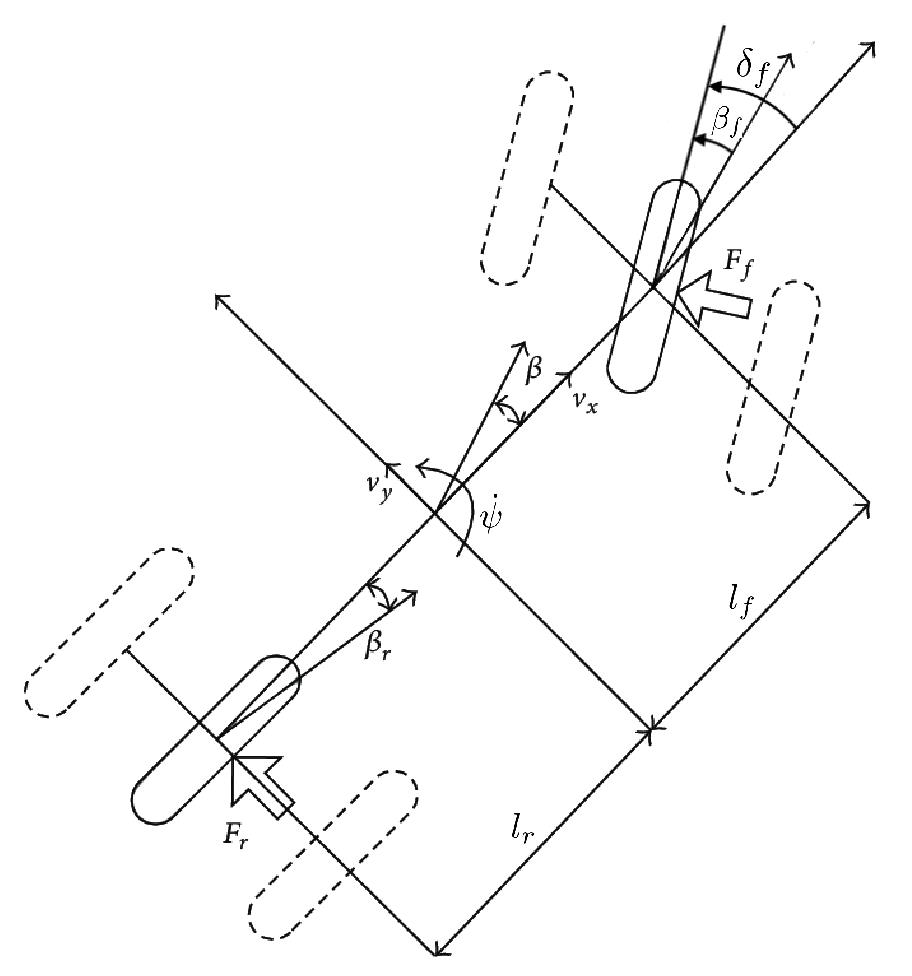
\includegraphics{image/single track model.jpeg}
    \caption{Single Track Model.}
    \label{fig:single_track}
\end{figure}

\noindent\textbf{Vehicle variables:}
\begin{itemize}
    \item $\delta_f$: steering angle.
    \item $\beta$: vehicle sleep angle $=$ angle between the vehicle longitudinal axis and velocity.
    \item $\beta_f, \beta_r$: tire slip angles $=$ angles between the tire longitudinal axis and velocity.
\end{itemize}

\noindent\textbf{Vehicle parameters:}
\begin{itemize}
    \item \acs{CoG}: center of gravity
    \item $m, J$: mass and moment of inertia
    \item $l_f$: distance \acs{CoG} -- front wheel center
    \item $l_r$: distance \acs{CoG} -- rear wheel center
    \item $c_f, c_r$: front/rear cornering stiffnesses.
\end{itemize}

\begin{figure}[htbp]
    \centering
    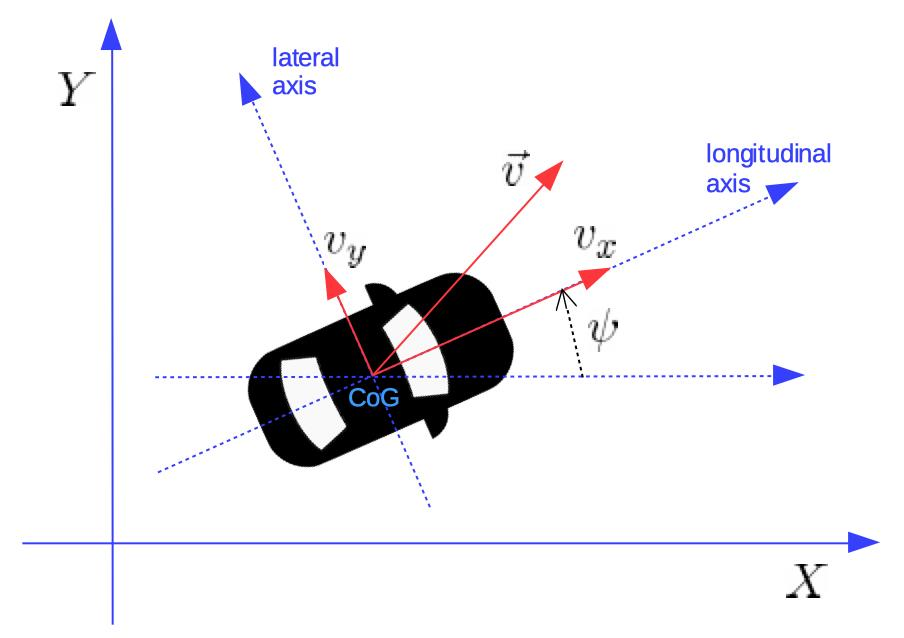
\includegraphics{image/vehicle reference system.jpeg}
    \caption{Vehicle Reference System.}
    \label{fig:Vehicle_reference}
\end{figure}

\noindent\textbf{Vehicle Dynamic parameters:}
\begin{itemize}
    \item $X, Y$: coordinates of the vehicle \acs{CoG} in an inertial reference frame (shown in Figure~\ref{fig:Vehicle_reference})
    \item $\psi$: yaw angle
    \item $\omega_\psi = \dot{\psi}$: yaw rate
    \item $\vec{v} \equiv V$: velocity vector in the inertial frame
    \item $v_x$: longitudinal speed $= \vec{v}$ component along the longitudinal axis
    \item $v_y$: lateral speed $= \vec{v}$ component along the lateral (transverse) axis
    \item $a_x$: longitudinal acceleration in the inertial frame.
\end{itemize}

The state equations of the \acs{DST} model are:
\begin{align}
    \dot{X}           &= V_x \cos\psi - V_y \sin\psi \\
    \dot{Y}           &= V_x \sin\psi + V_y \cos\psi \\
    \dot{\psi}        &= \omega_\psi \\
    \dot{V}_x         &= V_y \omega_\psi + a_x \\
    \dot{V}_y         &= -V_x \omega_\psi + \frac{2}{m}\left(F_{yf} + F_{yr}\right) \\
    \dot{\omega}_\psi &= \frac{2}{J}\left(l_f F_{yf} - l_r F_{yr}\right)
\end{align}

where $F_{yf}$ and $F_{yr}$ are the lateral forces exchanged between tire and road.

For the tire model, there are several tire model options:

\medskip
\noindent\textbf{Linear (for $V_x = \mathrm{const}$) tire model:}
\begin{equation}
    F_{yf} = -C_f \beta_f, \hspace{1.5em} F_{yr} = -C_r \beta_r
\end{equation}
\begin{equation}
    \beta_f = \frac{V_y + l_f \omega_\psi}{V_x} - \delta_f, \hspace{1.5em} \beta_r = \frac{V_y - l_r \omega_\psi}{V_x}
\end{equation}

\noindent\textbf{Nonlinear simplified tire model:}
\begin{equation}
    F_{yf} = -C_f \beta_f \cos\delta_f, \hspace{1.5em} F_{yr} = -C_r \beta_r
\end{equation}
\begin{equation}
    \beta_f = \arctan\!\left(\frac{V_y + l_f \omega_\psi}{V_x}\right) - \delta_f, \hspace{1.5em} \beta_r = \arctan\!\left(\frac{V_y - l_r \omega_\psi}{V_x}\right)
\end{equation}

\noindent\textbf{Nonlinear Pacejka tire model:}
\begin{equation}
    F_{yf} = -f_p(\beta_f)\cos\delta_f, \hspace{1.5em} F_{yr} = -f_p(\beta_r)
\end{equation}
where $\beta_f$ and $\beta_r$ and $f_p(\beta)$ is given by the Pacejka magic formula.

\noindent\textbf{Pacejka magic formula:}
\begin{equation}
    f_p(\beta) = p_1 \sin\!\big(p_2 \arctan\big(p_3 \beta - p_4(p_3 \beta - \arctan(p_3 \beta))\big)\big)
\end{equation}
$p_1$: peak value, $p_2$: shape factor, $p_3$: stiffness factor, $p_4$: curvature factor. Linearizing this formula, we find $p_1 p_2 p_3 = C_f$ (or $C_r$).

\begin{figure}[htbp]
    \centering
    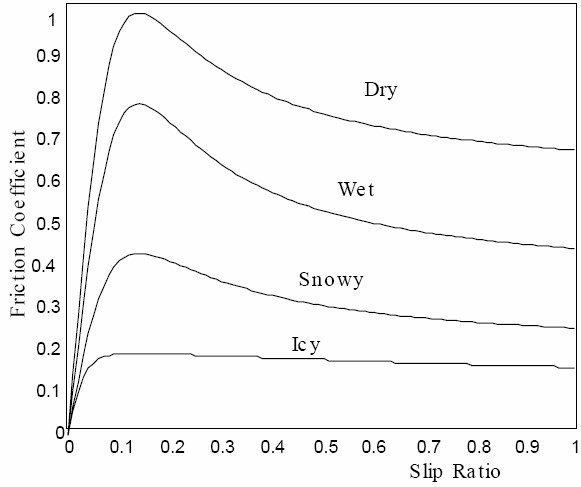
\includegraphics{image/friction coef.jpeg}
    \caption{Friction Coefficients in different conditions.}
    \label{fig:friction_coef}
\end{figure}

In the real world conditions, these parameters are really hard to measure or estimate because they change based on the road conditions (see Figure~\ref{fig:friction_coef}).

The real parameters of the vehicle in the simulation environment have been found with the help of Carla's \texttt{Vehicle.physics} command.

\medskip
\noindent\textbf{Vehicle Parameters Values}
\begin{itemize}
    \item $m$: 1318\,kg
    \item $J$: 2500\,kg/m\textsuperscript{2}
    \item $l_f$: 1.54\,m
    \item $l_r$: 1.51\,m
    \item $c_f$: 15000\,N/rad
    \item $c_r$: 15000\,N/rad
\end{itemize}

\subsection{Dispatching To Obtain Throttle-Brake Value From Acceleration Value}
To control a vehicle in the Carla simulator, we need three pieces of information: steering angle, throttle, and brake commands. However, our model generates $a_x$ data. It is not possible to directly provide this data to Carla because this information only tells us about the acceleration or deceleration of the vehicle and the magnitude of these changes. Therefore, we need to scale this data to use it for throttle-brake information. To do this, we perform dispatching. In the context of control, \enquote{dispatching} usually refers to the process of distributing tasks or resources according to certain criteria or algorithms.

To accomplish this, we first need specific reference values. These reference values should be collected according to many different scenarios to ensure they are suitable for every scenario, not just one. In our case, data were collected for three different scenarios: when the vehicle completes a straight path in a sine wave pattern, when continuous braking and accelerating are performed on a straight road, and finally, when only accelerating is done and the vehicle slows down without braking due to its own weight. The data include the vehicle's $a_x$ acceleration value, and throttle and brake values. By examining these accelerations, the priorities of throttle and brake values are determined for acceleration and deceleration situations. For instance, it is not always necessary to brake for negative acceleration values; reducing the throttle can also achieve the necessary speed reduction. Therefore, each value has its weight. Also, there is a range within which each command should be applied. These ranges can be determined using an if/else structure based on the acceleration value. The commands to be applied within these ranges are found by dividing the $a_x$ value by certain weight values. Consequently, the throttle and brake values are instantaneously derived from the $a_x$ value and provided to the vehicle in the Carla environment for application. As explained above, these values were found by analyzing reference data and through trial and error. The code for the if/else structure that creates the intervals for applying these values and commands is provided below.

\section{Data Gathering with Autonomous Driving Mode}
A reference point was selected from the Carla Map to collect reference data. The vehicle was spawned at this reference point. A simulation duration was determined based on a finish point we had predetermined. The vehicle was moved using Carla's autonomous driving mode. During this time, the necessary reference position, waypoint data, yaw angle, and speed data were recorded into a \texttt{.csv} file at intervals of $T_s = 0.05$ seconds. Once the required simulation duration was completed, the vehicle was removed from the map.
\hyphenation{}
Two collector routines are used during the recording. The first one, \texttt{carla\_data\_collector}, queries the full localization information of the vehicle at every tick: world position $(x, y, z)$, rotation (pitch, yaw, roll), linear velocity, linear acceleration and angular velocity. The second one, \texttt{carla\_data\_collector\_2}, focuses on the geometry of the lane and returns, for each tick, the position of the closest waypoint together with the unit forward vector $\hat{t} = (t_x, t_y)$ tangent to the lane in the legal direction of travel. The two collectors are complementary: the first one captures the dynamic state of the ego vehicle, the second one captures the geometric reference that the lane-keeping controller will track. The complete listings of both routines are reported in Appendix~\ref{app:b} for completeness; here we only describe the meaning of the recorded fields.

In order to keep the resulting \texttt{.csv} file compact, the second collector is wrapped by a duplicate-suppression block. The position of the closest waypoint can remain unchanged for several consecutive ticks---for instance when the vehicle stops at a traffic light---and writing identical rows to the file would simply increase its size without adding information. The block compares each new sample with the last one written and appends it only if at least one of the two coordinates has changed. The resulting file therefore contains a strictly monotonic sampling of the center line, indexed by the order in which the waypoints were visited.

\section{Data Gathering with Manual Driving Mode}
The first capability that we demonstrate with CARLA is localization, which allows our ego-vehicle to determine its pose in the world. Two coordinate frames: the map frame, which is a coordinate frame that is fixed at the initial position of the map, and the vehicle frame, which is a coordinate frame attached to the middle of the rear axle of the vehicle. For our particular experiment, we record the vehicle's accurate pose while traversing a curved-straight route in the Town10. In the Python API, there is a class that comprises all the localization information for an actor at a certain moment in time; its methods comprise Getters such as \texttt{get\_acceleration}, \texttt{get\_velocity}, \texttt{get\_transform}, and \texttt{get\_angular\_velocity}---which in our case we utilize the \texttt{get\_transform} method which includes both location of the object ($X$, $Y$, $Z$ from the origin of the map) in meters, and its rotation characteristics from which we utilize the yaw values. More concisely, $X$ and $Y$ coordinates were our focus, as in the map chosen, the road is entirely flat. Hence only these two coordinates remain crucial for tracking the vehicle's trajectory. Also, the Yaw angle, describing the orientation of the map's coordinate system, is essential for indication of the direction the vehicle is facing. Therefore for curved paths, which our scenarios contain, it is important.

Some additional considerations also are to be noted, such as the sampling rate, which determines the time step of the data collection. We have chosen $0.1$, indicating not too sparse to miss some critical dynamics, especially for sharp turns, and also not too frequent leading to redundant information.

After initializing the scenario and ego vehicle (based on the preferences), based on the duration of the scenario depending on the controls of the car (throttle, brake, and steering commands), we record the data of the vehicle at each time step. The corresponding logging routine has the same overall structure as in the autonomous mode---at every simulation tick the snapshot frame, the pose, the velocity, the acceleration and the applied control are appended to a Pandas dictionary which is finally written to disk as a \texttt{.csv} file. The full code excerpt is provided in Appendix~\ref{app:b}.
\hyphenation{}
In manual driving mode, the autopilot is disengaged with \texttt{vehicle.set\_autopilot(False)} and the user is given full control of throttle, brake, and steering through the keyboard. Each pressed key is captured as a PyGame event and is translated into a \texttt{carla.VehicleControl} object that is then applied to the ego vehicle in the simulator. While the user drives, the same getters introduced for the autonomous mode are queried at every simulation tick, so that the resulting \texttt{.csv} file shares the same structure for both modes and can be loaded by the controller without any additional preprocessing.

This dual-mode acquisition serves two purposes. First, it provides reference trajectories for the dispatcher tuning and for the controller design, since the autonomous mode of CARLA produces well-formed paths along the center of the lane. Second, it allows the recording of edge cases that are hard to reproduce automatically---for example aggressive lane changes, harsh braking, or following curves at the limit of stability---because they can be performed deliberately by a human driver. The two \texttt{.csv} files are then used as the input data set for the \ac{LKA} controller described in Chapter~\ref{ch3}.